%%% template.tex
%%%
%%% This LaTeX source document can be used as the basis for your technical
%%% paper or abstract. Intentionally stripped of annotation, the parameters
%%% and commands should be adjusted for your particular paper - title, 
%%% author, article DOI, etc.
%%% The accompanying ``template.annotated.tex'' provides copious annotation
%%% for the commands and parameters found in the source document. (The code
%%% is identical in ``template.tex'' and ``template.annotated.tex.'')

\documentclass[annual]{acmsiggraph}
\usepackage{program}

\TOGonlineid{45678}
\TOGvolume{0}
\TOGnumber{0}
\TOGarticleDOI{1111111.2222222}
\TOGprojectURL{}
\TOGvideoURL{}
\TOGdataURL{}
\TOGcodeURL{}

\title{Mobile Depth from Focus and Applications}

%\author{Naran Bayanbat\thanks{e-mail:naranb@stanford.edu}\\Stanford University \and Jason Chen\thanks{e-mail:jasonch@stanford.edu} \\Stanford University \and Chun-Wei Lee\thanks{e-mail:chunweil@stanford.edu} \\Stanford University}
\author{Naran Bayanbat\\naranb@stanford.edu\\Stanford University \and Jason Chen\\jasonch@stanford.edu\\Stanford University \and Chun-Wei Lee\\chunweil@stanford.edu\\Stanford University}
\pdfauthor{Naran Bayanbat, Jason Chen, Chun-Wei Lee}

\keywords{depth from focus, depth map, tablet, computational photography}

\begin{document}

 \teaser{
   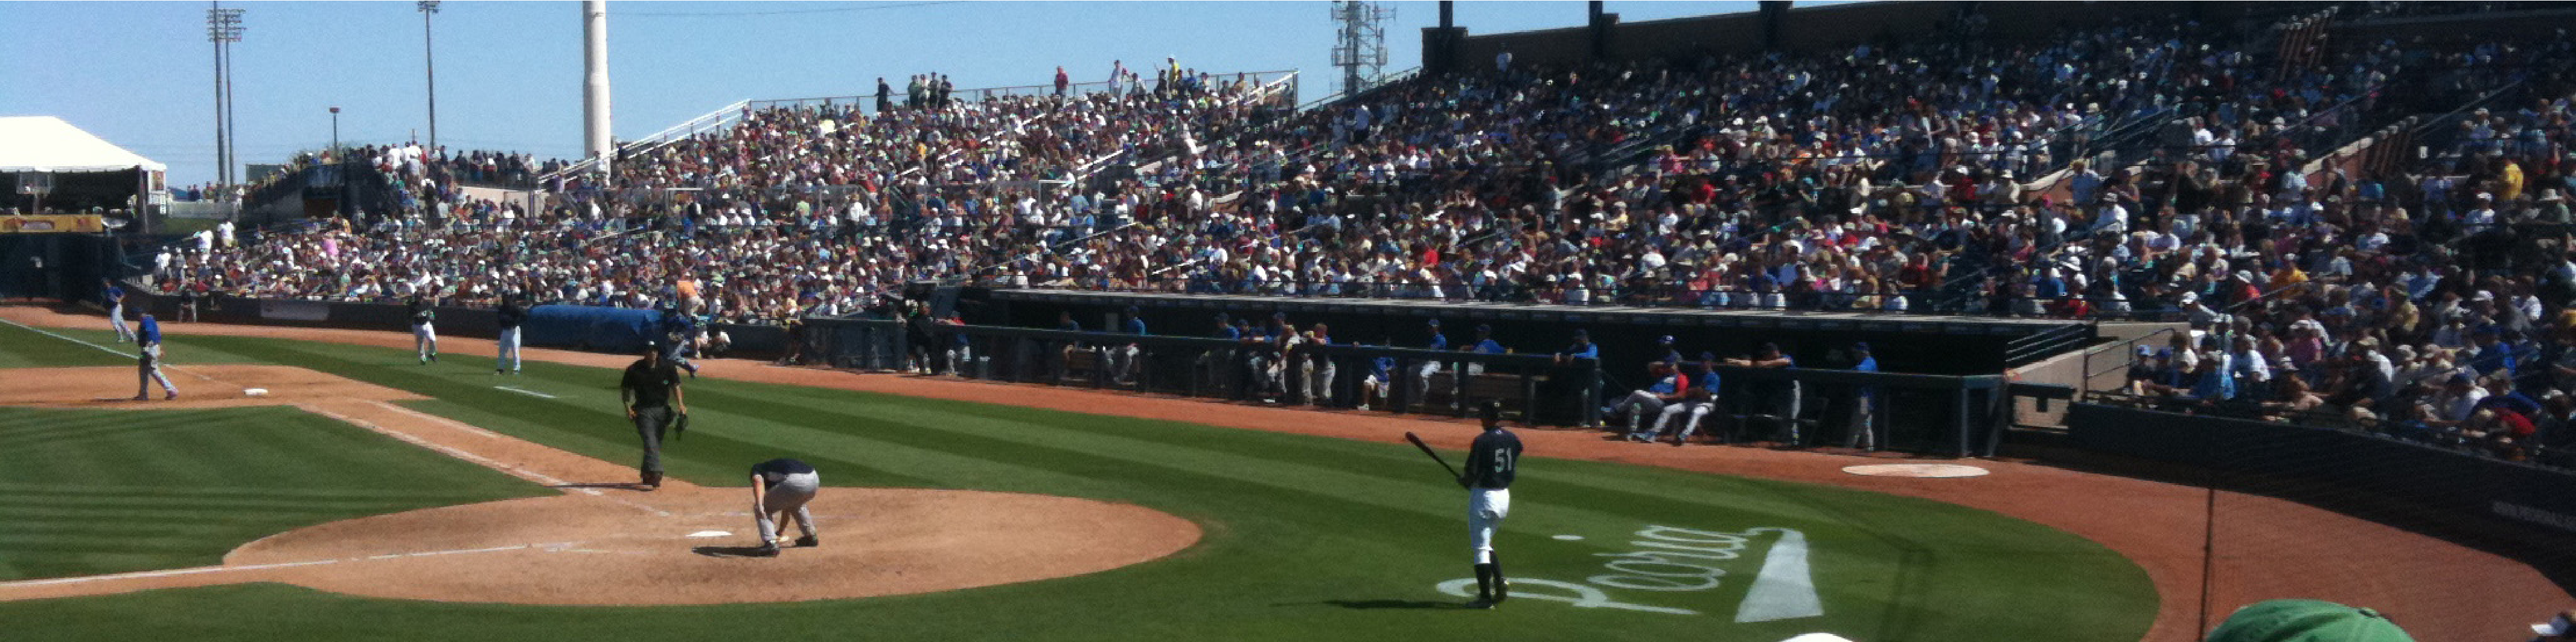
\includegraphics[height=1.5in]{images/sampleteaser}
   %\caption{}
 }

\maketitle

\begin{abstract}
Depth information is crucial in providing scene understanding for many post-processing applications in computational photography. While depth maps can be easily obtained through stereo cameras or external devices such as infrared sensors, it is difficult in mobile photography because of hardware limitation. In this project, we will implement depth-by-focus, sweeping a single lens across various focus distances and composite an approximate depth map. The depth map will be improved by segmentation and bilateral filtering. We will then demonstrate the effectiveness of the technique by utilizing the depth map and simulate light-field photography as well as synthetic depth of field.

\end{abstract}

\begin{CRcatlist}
  %\CRcat{I.3.3}{Computer Graphics}{Three-Dimensional Graphics and Realism}{Display Algorithms}
  %\CRcat{I.3.7}{Computer Graphics}{Three-Dimensional Graphics and Realism}{Radiosity};
\end{CRcatlist}

\keywordlist

%\TOGlinkslist

\copyrightspace

\section{Introduction}

Mobile devices have become the most common photography means, and they have presented a new set of opportunities and challenges for computational photography.  While many applications take advantage of these devices' location, accelerameter, and other meta data, the inherent hardware limitation on size computation power makes it worth revisiting prior works on computational photography to this application.  Specifically, since depth information is one of the most useful piece of scene understanding, we wish to demonstrate a mobile solution producing a depth map that assist in computational photography.  Since most mobile devices have only one camera (lens) and no active focusing equipment, we will attempt to implement depth from focus, approximating depth information from images captured at different depths. 

\section{Prior Work}

Depth from Focus is a technique that has been studied for decades \cite{Grossmann1987} and with numerous applications \cite{mobileRobot}.  ...

\section{Results}

\subsection{Depth Sampling}
At each focus distance, we densely sampled 36x27 patches ...    sobel filter... threshold...

\subsection{Depth Map Generation}

One of the inherent problem in sharpness calculations, as well as in all focusing methods in general, is that they fail on textureless surfaces.  Therefore, after obtaining the best focus distance and best sharpness pair, $<d_i, \lambda_i>$, for each sample point, we first correct for points sampled at low texture patches.  Every sample point whose sharpness is below some predefined threshold, $\Lambda$, will update its sharpness by finding the most common depth value in the patches around it.  This is achieved by a simple voting scheme: each of the nine pixels will cast a vote for the depth value it represents, and its vote is weighted by its confidence, which is the normalized sharpness value. \\
Then, we simply naively assume the entire patch exists at the same depth, thus generating a blocky depth map as in ~\ref{fig:initial-depth-map} of the same dimension as the input image. Next, we take a full-colored frame from the input stack as reference image, and use joint bilateral filtering to smooth out the patch boundaries.  This is because we want fairly aggressive smoothing while preserving edges from the color space. \\
This gives us our first approximate depth map, as shown in ~\ref{fig:filtered-depth-map}.  We quickly realized that any frame we could choose from the stack could not serve as a good edge reference, because at least some part of the image is out of focus.  We can solve the problem if we had an all-in-focus image, but we could only get a good all-in-focus image if we had a better depth map.  To solve this problem, we iteratively refined our depth map by generating all-in-focus image based on the current depth map ~\ref{fig:depth-map-refining}.  This provides us highly accurate depth map with clear object edges.

\subsection{All-in-Focus Imaging}

\subsubsection{Calibration}


\subsection{Synthetic Depth of Field Application}
\subsubsection{Image Merging}

Depth map provides us information estimated depth distances of the image pixels. Thus, when merging two images, we could get the information which objects in the images is in the front-focus, and could cover the scene of the another image from another image. The application is aimed to merge two images, which has all-in-focus image and depth map. We also assuming that there is no movement and position shift when taking these two images, so that the background is identical. The only difference is the front-focused objects. By utilizing the refined all-in-focus images and depth maps for each image, we simply choose each pixel to present by the corresponding depth value from the depth map. Comparing the depth value, we can synthesize a new image with both front-focused objects shown. 

The result is mainly depended on the quality of depth map.  The following images demonstrate a set of images and their merged image. When depth map value we estimated is accurate. The quality of image merging is well. 
\begin{figure}[h!]
   \centering
   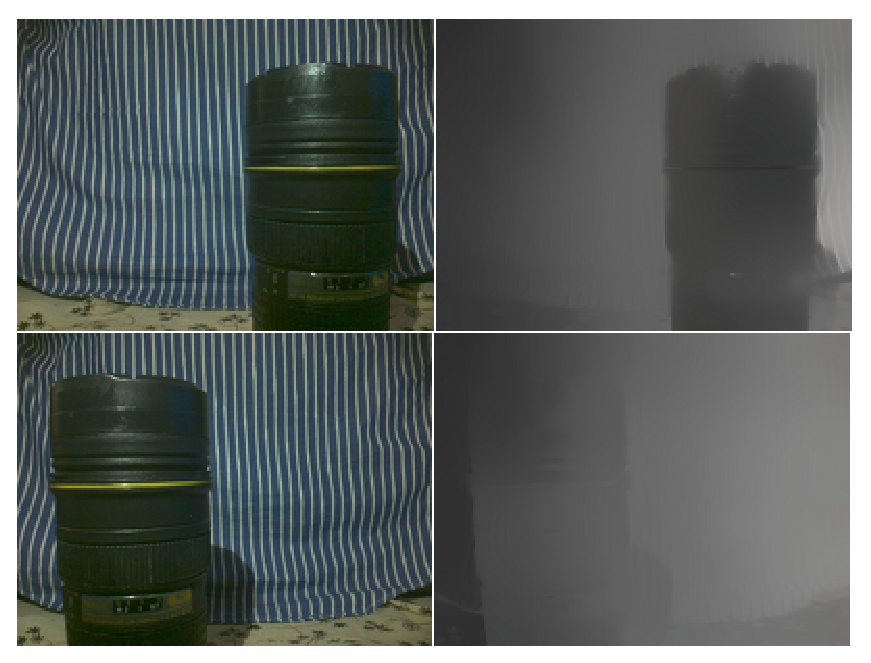
\includegraphics[height=2.0in]{images/merged1}
   \caption{Example set:Upper and lower left: all-in-focus images, and upper and lower right: the corresponding depth map. }
\end{figure}

\begin{figure}[h!]
   \centering
   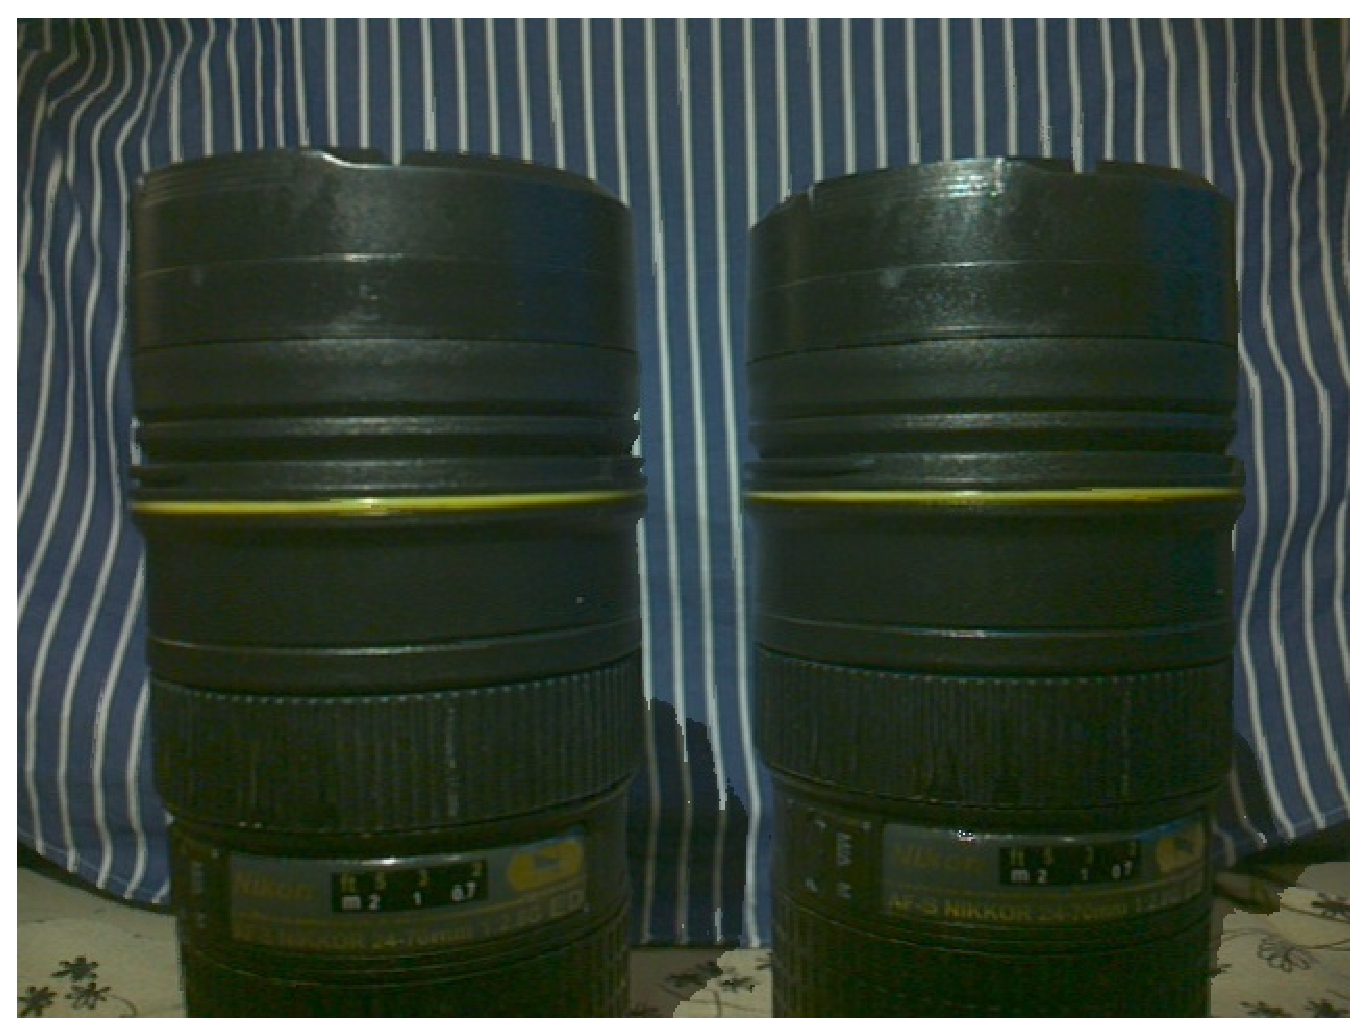
\includegraphics[height=2.0in]{images/merged}
   \caption{Example result: merged image}
\end{figure}

 There is some case that for one pixel, both images have the same depth value. The way we solve this issue now is choosing pixel of one image when this case occurs. 

\subsubsection{Image Depth of Field Image}

\section{Concolusions and Further Works}


For the imaging merging part, we need to using image segmentation to solve the ambiguity caused by the case that two images have the same depth value for one pixel. With assistance of image segmentation. we can choose the more likely image to present even if both images have the same depth value. 

\begin{figure}[h!]
   \centering
   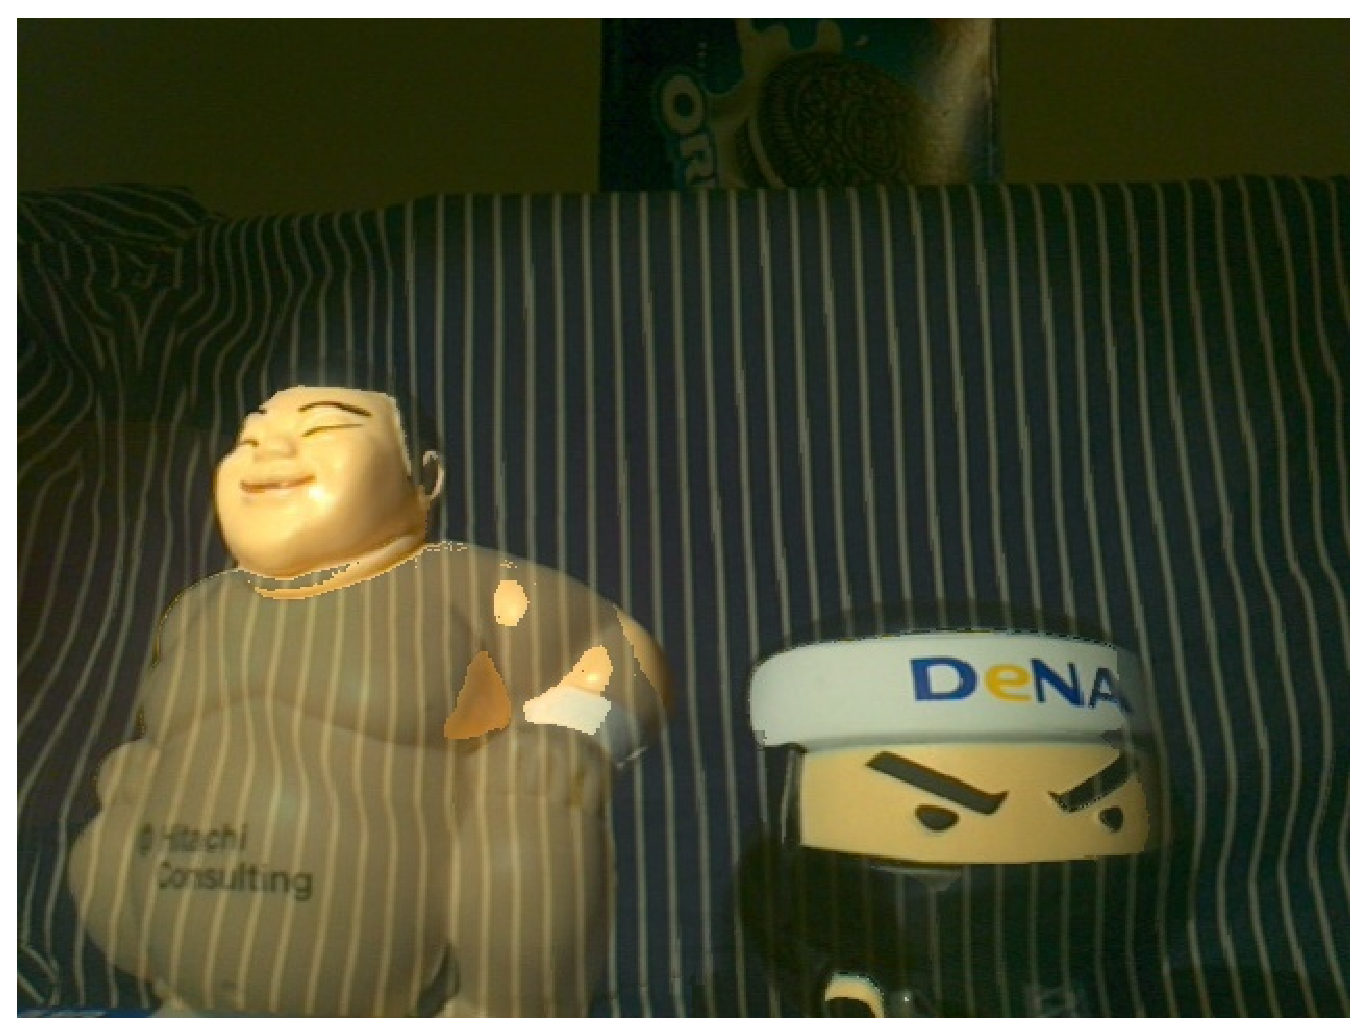
\includegraphics[height=2.0in]{images/faultmerged}
   \caption{Fault image: the semi-transparant parts are the areas have the same depth value in both depth values}
\end{figure}


\subsection{Lighting and Shadows}

\section*{Acknowledgements}


\bibliographystyle{acmsiggraph}
\bibliography{template}
\end{document}
